\documentclass[10pt, notitlepage,a4paper]{article}
\usepackage[margin=0.9in]{geometry}
\usepackage[T1]{fontenc}
\usepackage[utf8]{inputenc}
\usepackage[english, polish]{babel}
\let\babellll\lll
\let\lll\relax
\usepackage{amssymb,url}
\usepackage{ntheorem,tikz}
\usepackage{graphicx,lmodern}
\newcommand*\ruleline[1]{\par\noindent\raisebox{.8ex}{\makebox[\linewidth]{\hrulefill\hspace{1ex}\raisebox{-.8ex}{#1}\hspace{1ex}\hrulefill}}}
\pagestyle{empty}
%----------------------Marginesy------------
\setlength{\parindent}{0mm}
\setlength{\parskip}{2mm}

\newcommand{\N}{\mathbb{N}}
\newcommand{\xdotminus}[2]{%
  \ooalign{\hidewidth$\vcenter{\hbox{$#1\dot{}$}}$\hidewidth\cr$#1-$\cr}%
}
\providecommand{\dotminus}{\mathbin{\mathpalette\xdotminus\relax}}

%%%%%%%%%%%%%%%%%%
\theoremheaderfont{\normalfont\bfseries}
\theoremseparator{.}
\theorembodyfont{\normalfont\upshape}
\theoremstyle{plain}

\theoremindent1em
\newtheorem{zadanie}{Zadanie \hspace{-0.4em}}

\newtheorem{zadanieW}{Zadanie W\hspace{-0.4em}}  

 \pagestyle{plain}



\begin{document}
% \begin{comment}

\setcounter{section}{1}
\section*{Podstawowy warsztat informatyka --- lista 8}
\begin{zadanie} (1 punkt)
Wejdź na stronę:\\ \url{https://github.com/microsoft/Bringing-Old-Photos-Back-to-Life}\\ Obejrzyj otwarte i zamknięte pull requesty. Co robi microsoft-cla bot? Znajdź ,,Network graph'': jak są na nim zaznaczone pull requesty? 

Na koniec obejrzyj plik README.md. Podobnego pliku będziemy oczekiwać w każdym projekcie.
\end{zadanie}

\begin{zadanie} (1 punkt) To zadanie nie wymaga wcześniejszej znajomości języka Prolog ani algorytmu quicksort. Wystarczy wiedzieć, że na pracowniach jest zainstalowany interpreter Prologa, który można odpalić poleceniem swipl,
a kod w Prologu to ciąg klauzul. Klauzule są typowo postaci:
\begin{verbatim}
wniosek :- przeslanka1, ..., przeslankan.
\end{verbatim}
Taka linia odpowiada implikacji $przeslanka1 \wedge \dots \wedge przeslankan \Rightarrow wniosek$.

Ściągnij repozytorium \url{https://github.com/j-michaliszyn/quicksort17/}. Reprezentuje ono historię pewnej wadliwej implementacji algorytmu quicksort w języku Prolog. Twoim zadaniem będzie poprawić tę implementację (nie znając Prologa ani quicksorta). W tym celu:
\begin{enumerate}
\item Przejrzyj historię commitów. Znajdź (na podstawie opisów) taki, który jest jasnym oszustwem polegającym na usunięciu testu, który nie działa.
\item Ściągnij wcześniejszą wersję i sprawdź, czy rzeczywiście odpalenie programu z testami (poleceniem opisanym w README.md) zwraca informację, że jeden z testów nie jest spełniony.\\
\emph{Uwaga: Ten test jest zrandomizowany i z małym prawdopodobieństwem może być spełniony, więc lepiej uruchomić go dwa razy. Stąd wziął się cały problem -- w czasie edycji, która wprowadziła błąd, akurat przypadkiem test przeszedł.}
\item Pobieraj coraz to wcześniejsze wersje tego programu aż dojdziesz do takiej, gdzie oba testy są spełnione. Wywnioskuj (na podstawie opisu kolejnego commita), co zostało popsute i jak to naprawić.
\item Ściągnij jeszcze raz najnowszy commit i napraw program. Przywróć wcześniejszą wersję pliku z testami aby upewnić się, że wszystko działa.
\end{enumerate}
\end{zadanie}

\begin{zadanie}(2 punkty)
Jak już wiemy, jak naprawić błąd, to warto się to wiedzą podzielić i naprawić kod w oryginalnym repozytorium.  Oczywiście nie chcę dawać wszystkim studentom dostępu do pisania w moim repozytorium. Właśnie dla takich sytuacji jest zaprojektowany mechanizm Pull Request.

\begin{enumerate}
\item Utworzyć fork wspomnianego repozytorium i sklonować go na swój komputer, a następnie poprawić pliki w sposób opisany w poprzednim zadaniu.
\item  Stworzyć nowy commit oraz zrobić git push.
\item  Stworzyć pull request dotyczący dodania swojego commita do jedynej gałęzi w oryginalnym repozytorium.
\end{enumerate}
\end{zadanie}

\begin{zadanie} (3 punkty)
To zadanie należy wykonywać w parach. Jeśli nie masz pary, to zrób załóż sobie drugie konto na githubie i zrób wszystko samodzielnie...

Polecenia są podzielone na dwie osoby: A i E.
\begin{itemize}
\item[E] Utwórz jakieś niepuste repozytorium na githubie.
\item[A] Zrób forka tego repozytorium, wprowadź jakieś zmiany i przygotuj pull requesta.
\item[E] Skomentuj te zmiany i poproś o poprawki (Request changes).
\item[A] Wprowadź poprawki, zrób odpowiedni \verb+git commit --amend+, następnie spuszuj zmiany\footnote{To w zasadzie jest jedyna \emph{zwykła} sytuacja, w której wolno użyć git push -f --- gdy puszujemy do swojego roboczego forka. }.
\item[E] Zaakceptuj pull requesta, a następnie go scal używając ,,Squash  and merge''.
\end{itemize}

Następnie zamieńcie się rolami i powtórzcie eksperyment.
\end{zadanie}
\section*{Zadania bonusowe}

\begin{zadanie}(2* punkty)
Dowiedz się, jak działają hooki w gicie.
Stwórz hook (w dowolnym języku programowania, którego interpreter lub kompilator jest na pracowni), który sprawdza, czy podany opis commita ma co najwyżej 50 znaków w pierwszej linii. Jeśli nie, commit powinien zostać odrzucony ze stosowną informacją zwrotną. Przygotuj repozytorium do testowania i przeprowadź dwa testy sprawdzające działanie hooka: jeden z commitem z dobrym opisem, a drugi ze złym. 
\end{zadanie}

\begin{zadanie}(2* punkty) Dowiedz się, jak działa \texttt{git bisect}\footnote{git posiada dużo tego typu przydatnych narzędzi i nie ma sensu ich wszystkich omawiać na tym przedmiocie, więc przyglądamy się jednemu przykładowemu narzędziu.}. 
Przeprowadź eksperyment dotyczący \texttt{git bisect}. W tym celu stwórz skrypt (w dowolnym języku programowania), który:
\begin{itemize}
\item Utworzy puste repozytorium oraz doda do niego plik \verb+log+ o treści ,,Kolejne czasy:''.
\item Wylosuje liczbę $i$ między $1$ a $1024$.
\item Wykona $i-1$ razy operację \verb+ date >> log+
 a po niej \verb+git commit -a -m "Dodana data"+.
\item Wykona operację\footnote{
To ma oznaczać moment, w którym popełniono jakiś błąd.
} \verb+ date > log+
 a po niej \verb+git commit -a -m "Dodana data"+.
\item Wykona $1024-i$ razy operację \verb+ date >> log+
 a po niej \verb+git commit -a -m "Dodana data"+. 
\end{itemize}
Następnie wykorzystaj \verb+git bisect+ do znalezienia commita, w którym nastąpiło nadpisanie.
\end{zadanie}

\textbf{Uwaga: Do tego zadania trzeba zainstalować qemu i pobrać pół gigabajta danych.} \begin{zadanie} (2* punkty)
Użyj programu wget do ściągnięcia do katalogu \verb+/var/tmp+ pliku 
\url{ii.uni.wroc.pl/static/obraz.7z} 
zawierającego obraz pewnej instalacji Debiana. Ściągnięty plik rozpakuj i nazwij

\verb+debian-twoj_numer_indeksu.qcow2+

Uruchom pobrany obraz poleceniem

\verb+qemu-system-i386 -hda /var/tmp/debian-twoj_numer_indeksu.qcow2+

lub podobnym. Po kilku chwilach powinien powitać cię tekstowy ekran logowania. Niestety, nie znasz hasła roota. Co za pech.

Znajdź w internecie informację o tym, jak zmienić hasło roota i zmień je. To dużo łatwiejsze, niż by się mogło wydawać. Następnie uruchom system ponownie i zaloguj się na konto roota.

Ten system jest trochę nieaktualny. Dowiedz się, jak go zaktualizować programem \verb+apt-get+. Następnie zainstaluj program \verb+git+ i go uruchom.
\end{zadanie}



\begin{zadanie} (5* punktów) (termin oddania 21 grudnia g. 15:45 przez formularz \url{https://classroom.github.com/a/U_8h3BI6})
Pod adresem \url{https://iidle.herokuapp.com/} jest pewna gra, dotycząca naszych studiów. Gra ta, choć ciekawa, jest dość żmudna - wiele razy trzeba wysyłać ten sam formularz. Twoim zadaniem będzie automatyzacja grania w tę grę. \emph{Uwaga: To zadanie zostało napisane z wykorzystaniem przeglądarki Chrome. Pod Firefoksem jest niemal identycznie, a w innych przeglądarkach to nie wiem}.

Zapoznaj się z zasadami gry i pograj chwilę. Odkryjesz, że najbardziej uciążliwe jest wysyłanie planu dnia. Wejdź na stronę wysyłania planu, ale tym razem przed wysłaniem planu wciśnij F12, a następnie wybierz zakładkę ,,Network''\footnote{Oczywiście w innych wersjach językowych będzie się to inaczej nazywać.}. Wyślij plan, a następnie zaobserwuj, co się stało. Pojawiło się nowe żądanie. Kliknij to żądanie prawym przyciskiem myszki, a następnie wybierz ,,Copy as cURL''.  

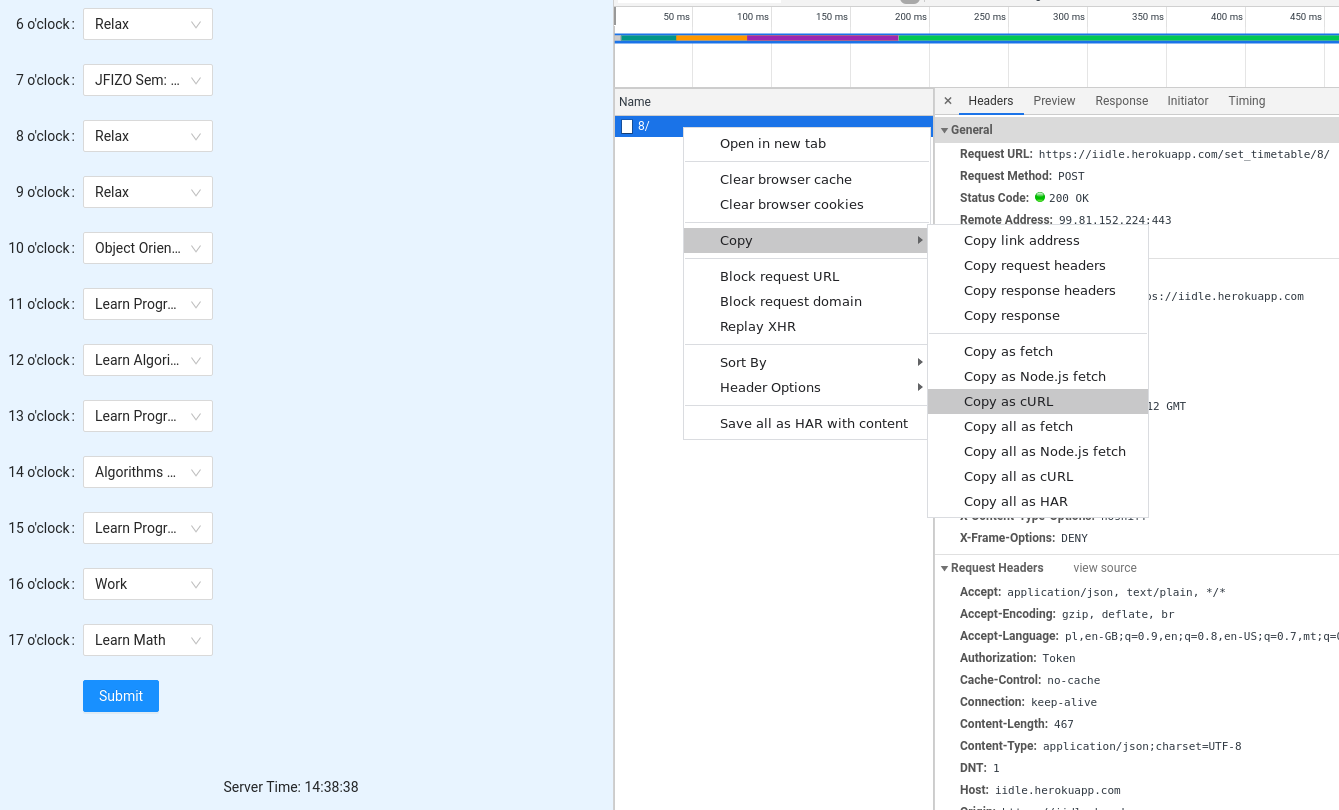
\includegraphics[scale=1.3]{iidle.png}

Wklej ten tekst do jakiegoś edytora tekstu -- jest to polecenie pozwalające wysłać, z pomocą programu cURL, plan do serwera gry. Stwórz na tej podstawie skrypt (w bashu, pythonie albo dowolnym innym języku) do grania w grę, który sam w odpowiednich odstępach czasu będzie wysyłał plany. 

To zadanie ma 2 wersje: w podstawowej, za 4 punkty, nie należy się martwić autoryzacją i można założyć, że skrypt działa tak długo, jak autoryzacja jest ważna (czyli po jakimś czasie serwer przestanie przyjmować żądania - wtedy trzeba będzie ręcznie skopiować nowy token autoryzacji). Aby dostać piąty punkt, należy dopisać zarządzanie logowaniem i odświeżaniem tokenów autoryzacji tak, by skrypt grał w grę zupełnie sam.
\end{zadanie}

\end{document}


\begin{zadanie}(2 punkty)
Święta minęły, czas usunąć choinkę. Twoim zadaniem będzie napisanie polecenia lub skryptu, który usunie wszystkie wystąpienia wyrazu ``choinka'' z pliku. Żeby zrozumieć, na czym polega trudność, rozpatrzmy takie podejście:

\begin{verbatim}
$ echo "zwykła choinka | nieusuwalna chochochoinkainkainka hahaha" > test.txt
$ sed 's/choinka//g' < test.txt 
zwykła  | nieusuwalna chochoinkainka hahaha
\end{verbatim}

Jak widać, wynik zawiera choinkę, a nie powinien. Zastanów się, jak sobie z tym poradzić i jaką złożoność mają możliwe rozwiązania. Następnie zaimplementuj (w czym chcesz, np. w bashu, sedzie, awku, pythonie, c++, lua, \dots) najlepsze z nich.
\end{zadanie}




